\chapter{Progettazione}

\section{Analisi}
  Questo capitolo ha come obiettivo quello di descrivere i requisiti che deve soddisfare e quindi
  le funzionalità che deve implementare la soluzione DLP oltre agli eventuali vincoli a cui deve attenersi.

  \subsection{Soluzione DLP per il traffico email}
  La soluzione DLP implementata va a proteggere i data-in-motion, più nello specifico
  si focalizza sulla protezione delle email. La soluzione monitora il traffico email e
  il loro contenuto in modo da:

  \begin{enumerate}
      \item {identificare la presenza di dati riservati al loro interno;}
      \item {prevenire l'invio, così da evitare la fuoriuscita dall’ambiente aziendale di queste informazioni.}
  \end{enumerate}

  \subsection{Motivazione scelta e obiettivo}
  La scelta di implementare questa funzionalità è dovuta al fatto che le email sono uno, 
  se non il principale, dei metodi di comunicazione in ambito aziendale.
  L’implementazione di questa funzionalità, oltre ad essere utile, risulta anche interessante.

  Lo scopo principale è quello di incrementare la sicurezza enterprise,  
  evitando la diffusione di dati riservati.

  \pagebreak
  \subsection{Glossario}
  Il glossario mostrato nella tabella \ref{Glossario} è una raccolta dei termini significativi, utilizzati 
  nel progetto, e delle relative definizioni.
  \begin{table}[!b]
      \centering
      \resizebox{\textwidth}{!}{%
      \begin{tabular}{|l|l|}
      \hline
      \rowcolor[HTML]{EFEFEF} 
      \textbf{Termine} &
        \textbf{Definizione} \\ \hline 
      Dipendente &
        \begin{tabular}[c]{@{}l@{}}Membro del personale. \\ Può essere il mittente o \\ il destinatario di una email.\end{tabular} \\ \hline 
      Mittente &
        \begin{tabular}[c]{@{}l@{}}Colui che invia la email.\\ Per questo progetto il mittente \\ è inteso come un dipendente \\ interno all’azienda.\end{tabular} \\ \hline
      Destinatario &
        \begin{tabular}[c]{@{}l@{}}Colui che riceve la email.\\ Può essere sia interno che \\ esterno all’azienda.\end{tabular} \\ \hline
      Email &
        \begin{tabular}[c]{@{}l@{}}Oggetto che va monitorato e \\ ispezionato dalla soluzione DLP.\\ In generale una email contiene:\\ -  Mittente;\\ -  Destinatario;\\ -  Oggetto;\\ -  Corpo;\\ -  Allegato (opzionale).\\ \\ I primi due attributi possono \\ essere oggetto di analisi del contesto, \\ mentre gli ultimi tre verranno ispezionati \\ durante l’analisi del contenuto.\end{tabular} \\ \hline
      Dati riservati &
        \begin{tabular}[c]{@{}l@{}}Dati che hanno maggior valore, ad esempio:\\ - dati di business\\  (contratti, proprietà intellettuale, progetti);\\  \\ - dati personali \\ (Codici fiscali, date di nascita \\ e altre informazioni sui dipendenti \\ e/o clienti);\\ \\ - dati finanziari \\ (dati della carta di credito o di altre modalità di pagamento);\\ eccetera.\end{tabular} \\ \hline
      \end{tabular}%
      }
      \caption{Glossario dei termini}\label{Glossario}
      \end{table}

      \pagebreak
      
      \subsection{Analisi dei requisiti}

        \subsubsection{Obiettivo utente:}
        La soluzione DLP deve identificare la presenza di dati/documenti riservati all’interno delle email 
        in modo da evitare che lascino il sistema aziendale.

        \subsubsection{Requisiti:}



        \begin{table}[htp]
            \centering
            \resizebox{\textwidth}{!}{%
            \begin{tabular}{ll}
            \multicolumn{2}{c}{requisito 1 (RF01): \textbf{Monitoraggio traffico SMTP}}                               \\ \hline
            \rowcolor[HTML]{EFEFEF} 
            \multicolumn{1}{|l|}{\cellcolor[HTML]{EFEFEF}ID}       & \multicolumn{1}{l|}{\cellcolor[HTML]{EFEFEF}RF01}           \\ \hline
            \multicolumn{1}{|l|}{Nome}                             & \multicolumn{1}{l|}{Monitoraggio traffico email (SMTP)}     \\ \hline
            \rowcolor[HTML]{EFEFEF} 
            \multicolumn{1}{|l|}{\cellcolor[HTML]{EFEFEF}Definizione} &
              \multicolumn{1}{l|}{\cellcolor[HTML]{EFEFEF}La soluzione deve monitorare il traffico email} \\ \hline
            \multicolumn{1}{|l|}{Motivazione} &
              \multicolumn{1}{l|}{\begin{tabular}[c]{@{}l@{}}Senza l'implementazione di questo requisito,\\ la soluzione non può funzionare. È il requisito\\ base per poter implementare gli altri\end{tabular}} \\ \hline
            \rowcolor[HTML]{EFEFEF} 
            \multicolumn{1}{|l|}{\cellcolor[HTML]{EFEFEF}Priorità} & \multicolumn{1}{l|}{\cellcolor[HTML]{EFEFEF}Indispensabile} \\ \hline
            \multicolumn{1}{|l|}{Dipendenze}                       & \multicolumn{1}{l|}{/}                                      \\ \hline
            \end{tabular}%
            }
            \newline
            \vspace*{1 cm}
            \newline
        \end{table}



        \begin{table}[htp]
            \centering
            \resizebox{\textwidth}{!}{%
            \begin{tabular}{ll}
            \multicolumn{2}{c}{requisito 2 (RF02): \textbf{Analisi del contenuto}}                                    \\ \hline
            \rowcolor[HTML]{EFEFEF} 
            \multicolumn{1}{|l|}{\cellcolor[HTML]{EFEFEF}ID}       & \multicolumn{1}{l|}{\cellcolor[HTML]{EFEFEF}RF02}           \\ \hline
            \multicolumn{1}{|l|}{Nome}                             & \multicolumn{1}{l|}{Analisi del contenuto}                  \\ \hline
            \rowcolor[HTML]{EFEFEF} 
            \multicolumn{1}{|l|}{\cellcolor[HTML]{EFEFEF}Definizione} &
              \multicolumn{1}{l|}{\cellcolor[HTML]{EFEFEF}\begin{tabular}[c]{@{}l@{}}La soluzione deve analizzare il contenuto di\\ ogni email che viene inviata.\end{tabular}} \\ \hline
            \multicolumn{1}{|l|}{Motivazione} &
              \multicolumn{1}{l|}{\begin{tabular}[c]{@{}l@{}}Senza l'implementazione di questo requisito,\\ La soluzione non sarebbe in grado di\\identificare contenuti riservati\end{tabular}} \\ \hline
            \rowcolor[HTML]{EFEFEF} 
            \multicolumn{1}{|l|}{\cellcolor[HTML]{EFEFEF}Priorità} & \multicolumn{1}{l|}{\cellcolor[HTML]{EFEFEF}Indispensabile} \\ \hline
            \multicolumn{1}{|l|}{Dipendenze}                       & \multicolumn{1}{l|}{RF01}                                   \\ \hline
            \end{tabular}%
            }
            \end{table}


        \begin{table}[htp]
            \centering
            \resizebox{\textwidth}{!}{%
            \begin{tabular}{ll}
            \multicolumn{2}{c}{requisito 3 (RF03): \textbf{Analisi del contesto}}                                                   \\ \hline
            \rowcolor[HTML]{EFEFEF} 
            \multicolumn{1}{|l|}{\cellcolor[HTML]{EFEFEF}ID}       & \multicolumn{1}{l|}{\cellcolor[HTML]{EFEFEF}RF03}                         \\ \hline
            \multicolumn{1}{|l|}{Nome}                             & \multicolumn{1}{l|}{Analisi del contesto}                                 \\ \hline
            \rowcolor[HTML]{EFEFEF} 
            \multicolumn{1}{|l|}{\cellcolor[HTML]{EFEFEF}Definizione} &
              \multicolumn{1}{l|}{\cellcolor[HTML]{EFEFEF}\begin{tabular}[c]{@{}l@{}}La soluzione, oltre ad analizzare il contenuto\\ di una email, deve anche tenere conto del \\ contesto\end{tabular}} \\ \hline
            \multicolumn{1}{|l|}{Motivazione} &
              \multicolumn{1}{l|}{\begin{tabular}[c]{@{}l@{}}Effettuare l'analisi del contesto può essere un\\ utile supporto all'analisi del contenuto.\end{tabular}} \\ \hline
            \rowcolor[HTML]{EFEFEF} 
            \multicolumn{1}{|l|}{\cellcolor[HTML]{EFEFEF}Priorità} & \multicolumn{1}{l|}{\cellcolor[HTML]{EFEFEF}Non Indispensabile, ma utile} \\ \hline
            \multicolumn{1}{|l|}{Dipendenze}                       & \multicolumn{1}{l|}{RF01}                                                 \\ \hline
            \end{tabular}%
            }
            \end{table}



        \begin{table}[htp]
            \centering
            \resizebox{\textwidth}{!}{%
            \begin{tabular}{ll}
            \multicolumn{2}{c}{requisito 4 (RF04): \textbf{Identificazione dati riservati}}                   \\ \hline
            \rowcolor[HTML]{EFEFEF} 
            \multicolumn{1}{|l|}{\cellcolor[HTML]{EFEFEF}ID}       & \multicolumn{1}{l|}{\cellcolor[HTML]{EFEFEF}RF04}           \\ \hline
            \multicolumn{1}{|l|}{Nome}                             & \multicolumn{1}{l|}{Identificazione di dati riservati} \\ \hline
            \rowcolor[HTML]{EFEFEF} 
            \multicolumn{1}{|l|}{\cellcolor[HTML]{EFEFEF}Definizione} &
              \multicolumn{1}{l|}{\cellcolor[HTML]{EFEFEF}\begin{tabular}[c]{@{}l@{}}La soluzione dev'essere in grado di identificare eventuali\\ dati/contenuti riservati presenti all'interno delle email\end{tabular}} \\ \hline
            \multicolumn{1}{|l|}{Motivazione} &
              \multicolumn{1}{l|}{\begin{tabular}[c]{@{}l@{}}Senza l'implementazione di questo requisito non è \\ possibile raggiungere l'obiettivo utente\end{tabular}} \\ \hline
            \rowcolor[HTML]{EFEFEF} 
            \multicolumn{1}{|l|}{\cellcolor[HTML]{EFEFEF}Priorità} & \multicolumn{1}{l|}{\cellcolor[HTML]{EFEFEF}Indispensabile} \\ \hline
            \multicolumn{1}{|l|}{Dipendenze}                       & \multicolumn{1}{l|}{RF01, RF02}                             \\ \hline
            \end{tabular}%
            }
            \end{table}


        \begin{table}[htp]
            \centering
            \resizebox{\textwidth}{!}{%
            \begin{tabular}{ll}
            \multicolumn{2}{c}{requisito 5 (RF05): \textbf{Azioni di risposta}}                         \\ \hline
            \rowcolor[HTML]{EFEFEF} 
            \multicolumn{1}{|l|}{\cellcolor[HTML]{EFEFEF}ID}       & \multicolumn{1}{l|}{\cellcolor[HTML]{EFEFEF}RF05}           \\ \hline
            \multicolumn{1}{|l|}{Nome}                             & \multicolumn{1}{l|}{Intraprendere azioni di risposta}       \\ \hline
            \rowcolor[HTML]{EFEFEF} 
            \multicolumn{1}{|l|}{\cellcolor[HTML]{EFEFEF}Definizione} &
              \multicolumn{1}{l|}{\cellcolor[HTML]{EFEFEF}\begin{tabular}[c]{@{}l@{}}La soluzione deve poter intraprendere una varietà di azioni:\\ 1. consentire l’invio;\\ 2. bloccare l’invio;\\ 3. eliminare il contenuto riservato e procedere con l’invio.\end{tabular}} \\ \hline
            \multicolumn{1}{|l|}{Motivazione} &
              \multicolumn{1}{l|}{\begin{tabular}[c]{@{}l@{}}Poiché la soluzione deve evitare che dati riservati \\ lascino il sistema aziendale, l'implementazione di questo \\ requisito è fondamentale\end{tabular}} \\ \hline
            \rowcolor[HTML]{EFEFEF} 
            \multicolumn{1}{|l|}{\cellcolor[HTML]{EFEFEF}Priorità} & \multicolumn{1}{l|}{\cellcolor[HTML]{EFEFEF}Indispensabile} \\ \hline
            \multicolumn{1}{|l|}{Dipendenze}                       & \multicolumn{1}{l|}{RF01, RF04}                             \\ \hline
            \end{tabular}%
            }
            \end{table}


        \begin{table}[htp]
        \centering
        \resizebox{\textwidth}{!}{%
        \begin{tabular}{ll}
        \multicolumn{2}{c}{requisito 6 (RF06): \textbf{Avviso in caso di blocco}}                                 \\ \hline
        \rowcolor[HTML]{EFEFEF} 
        \multicolumn{1}{|l|}{\cellcolor[HTML]{EFEFEF}ID}       & \multicolumn{1}{l|}{\cellcolor[HTML]{EFEFEF}RF06}           \\ \hline
        \multicolumn{1}{|l|}{Nome}                             & \multicolumn{1}{l|}{Avviso in caso di blocco}               \\ \hline
        \rowcolor[HTML]{EFEFEF} 
        \multicolumn{1}{|l|}{\cellcolor[HTML]{EFEFEF}Definizione} &
          \multicolumn{1}{l|}{\cellcolor[HTML]{EFEFEF}\begin{tabular}[c]{@{}l@{}}La soluzione deve sempre avvisare il mittente \\ in caso decida di bloccare l'invio della \\ email\end{tabular}} \\ \hline
        \multicolumn{1}{|l|}{Motivazione} &
          \multicolumn{1}{l|}{\begin{tabular}[c]{@{}l@{}}Utile avvisare il mittente in caso\\ sia necessario bloccare l'invio della sua email\end{tabular}} \\ \hline
        \rowcolor[HTML]{EFEFEF} 
        \multicolumn{1}{|l|}{\cellcolor[HTML]{EFEFEF}Priorità} & \multicolumn{1}{l|}{\cellcolor[HTML]{EFEFEF}Indispensabile} \\ \hline
        \multicolumn{1}{|l|}{Dipendenze}                       & \multicolumn{1}{l|}{RF05}                                   \\ \hline
        \end{tabular}%
        }
        \newline
        \vspace*{1 cm}
        \newline
        \end{table}

        \pagebreak
        \subsection{Dipendenze tra requisiti}
        Di seguito è stilato un elenco delle dipendenze formatesi tra i requisiti.
        La nomenclatura utilizzata è la seguente:
        \begin{flushleft}
          x -> y: il requisito x dipende dal requisito y
          \newline
          \newline
          RF02 -> RF01

          RF03 -> RF01

          RF04 -> RF01, RF02

          RF05 -> RF01, RF04

          RF06 -> RF05
          \newline
          \newline
          Elenco delle dipendenze semplificato: 
          \newline
          \newline
          RF02 -> RF01

          RF03 -> RF01

          RF04 -> RF02

          RF05 -> RF04 
          
          RF06 -> RF05
        \end{flushleft}

        \newpage
        \subsection{Grafo delle Dipendenze}
        Le dipendenze tra i requisiti formano un grafo aciclico, rappresentato nella figura \ref{grafoDipendenze}, che bisogna tenere in considerazione in caso si debba modificare uno dei requisiti del sistema.

        \begin{figure}[htp]
          \centering
          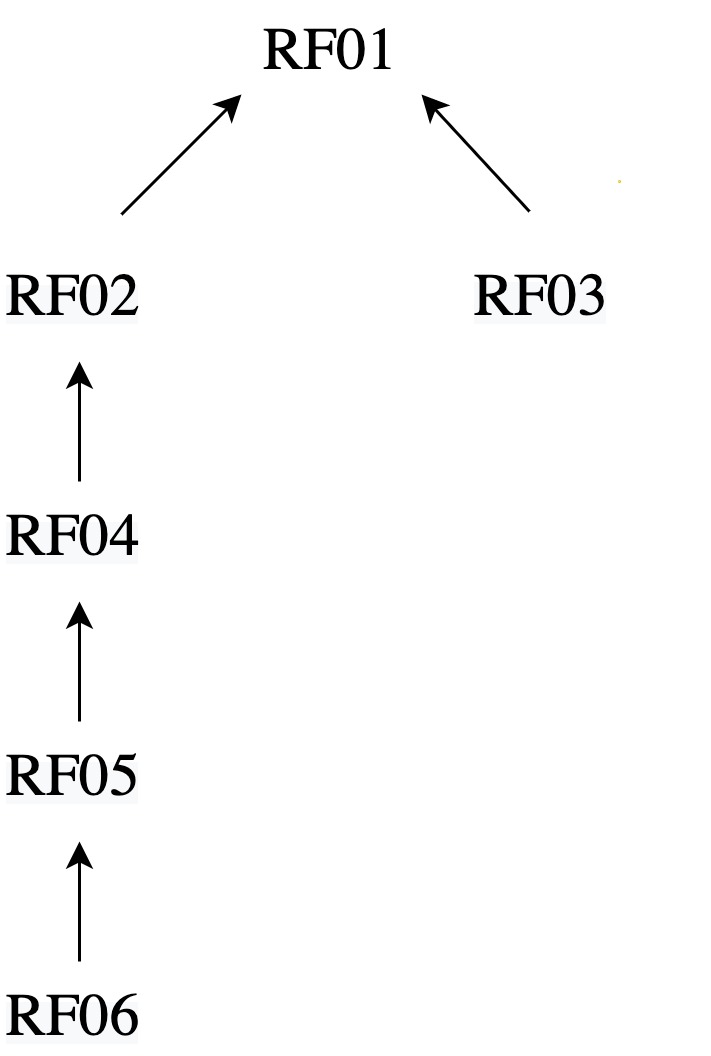
\includegraphics[width=.4\textwidth, height=.3\textheight, keepaspectratio]{grafo.jpg}
          \caption{Grafo aciclico delle dipendenze}\label{grafoDipendenze}
        \end{figure}

\section{Disegno dell'architettura}

  Per la progettazione della soluzione viene inserita la soluzione DLP,
  come mostrato in figura \ref{disegno1},
  tra il mail client (Outlook) e il mail server aziendale (Aruba). La soluzione DLP deciderà se consentire l'inoltro
  del messaggio verso il mail server aziendale, oppure bloccarne l'invio.
  \begin{figure}[htp]
    \centering
    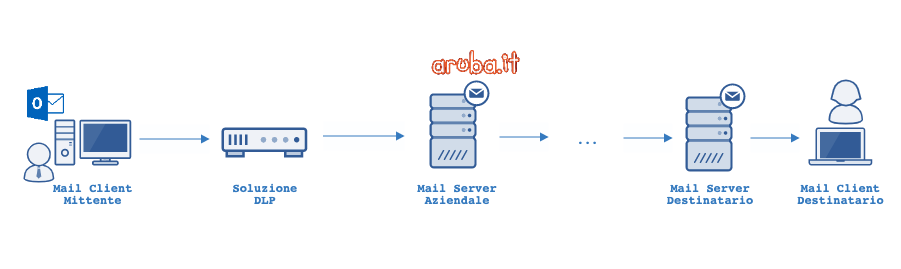
\includegraphics[width=12cm, height=16cm, keepaspectratio]{disegno1.png}
    \caption{disegno architettura per un mail client}\label{disegno1}
  \end{figure}

  \pagebreak
  La soluzione DLP è stata implementata attraverso l'uso di un mail server di inoltro (relay mail server).
  Il disegno subisce la seguente modifica mostrata in figura \ref{disegno2}.

  \begin{figure}[htp]
    \centering
    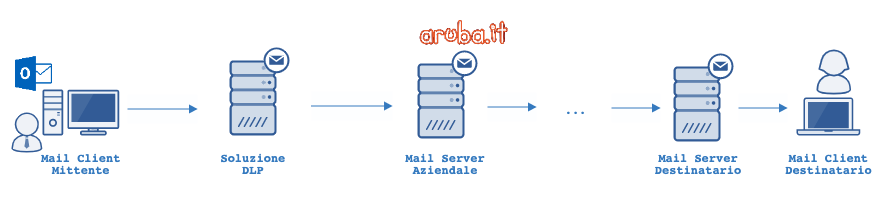
\includegraphics[width=12cm, height=16cm, keepaspectratio]{disegno2.png}
    \caption{soluzione DLP attraverso mail server di relay}\label{disegno2}
  \end{figure}

  Come ultimo passo si è andato a considerare una sottorete composta dagli host dei dipendenti dell'azienda, al
  posto di un unico client. La figura \ref{disegno3} mostra la configurazione risultante.

  \begin{figure}[htp]
    \centering
    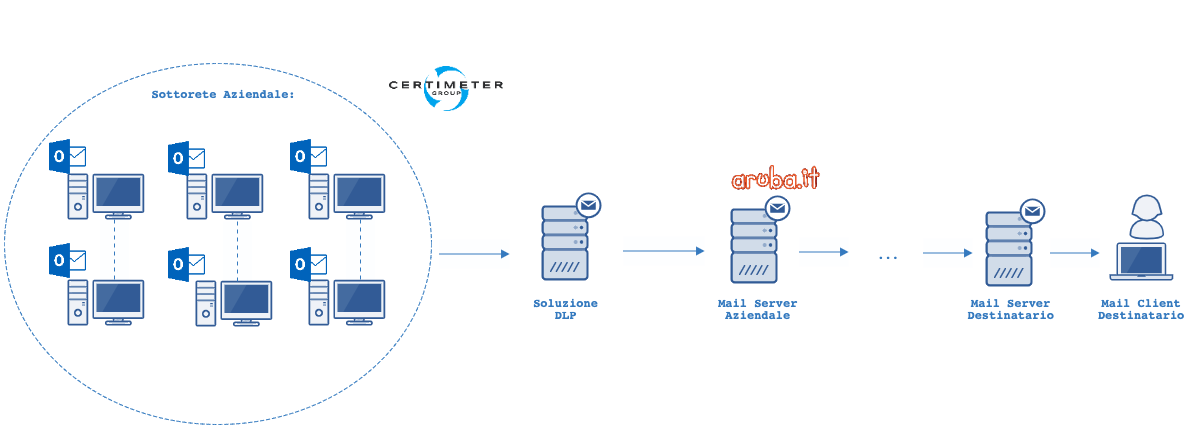
\includegraphics[width=12cm, height=16cm, keepaspectratio]{disegno3.png}
    \caption{soluzione DLP attraverso mail server di relay per una sottorete}\label{disegno3}
  \end{figure}

  \subsection{Descrizione del flusso di dati e di controllo}
  Come mostrato dalle figure \ref{disegno2} e \ref{disegno3}, quando un dipendente invia una email, questa
  passerà dal relay mail server che deciderà se bloccarla, oppure inoltrarla al mail server aziendale. L'email
  continuerà il suo cammino fino ad arrivare al mail server del destinatario. A quel punto potrà essere scaricata
  dal mail client del destinatario.